\documentclass[12pt]{article}
\usepackage{amsmath}
\usepackage{graphicx}
\usepackage{siunitx}
\usepackage{wrapfig}
\usepackage{multicol}
\usepackage{xcolor}
\usepackage[utf8]{inputenc}



\begin{document}


\title{Synchronus 4- bit Gray counter  \\ Lab Report 1 \\ ELP201}
\author{Deevyansh Khadria\\ 2022EE31883 }
\maketitle

\vspace{15px}
\tableofcontents






\newpage
\section{Aim}
    Stimulate a Gray Code-counter (synchronus) Using SR Flip 
\section{Apparatus}
    \begin{enumerate}
        \item Resistor
        \item Bread Board
        \item LED
        \item CPLD
        \item DC Source
    \end{enumerate}
\section{Theory}
    \begin{enumerate}
        \item A Gray Code counts in sucha mamer that difference between any two consecutive States differ by I bit
        \item The Counter starts with binary value co in must cases) and comeerts it to Gray Cadi. In boray Code, lach bit is determined by exclusive XOR of corresponding bits in binary representation The most significant bit (MSB) of gray code Is same as MSB of binary code.
        \item The main idea is to use SR Flip flop. we needed to design a circuit that can transition from one state to next in a gray code Sequence. Each flip-flop reforesent one bit in counter.
    \end{enumerate}

    
    \begin{figure}
        \centering
        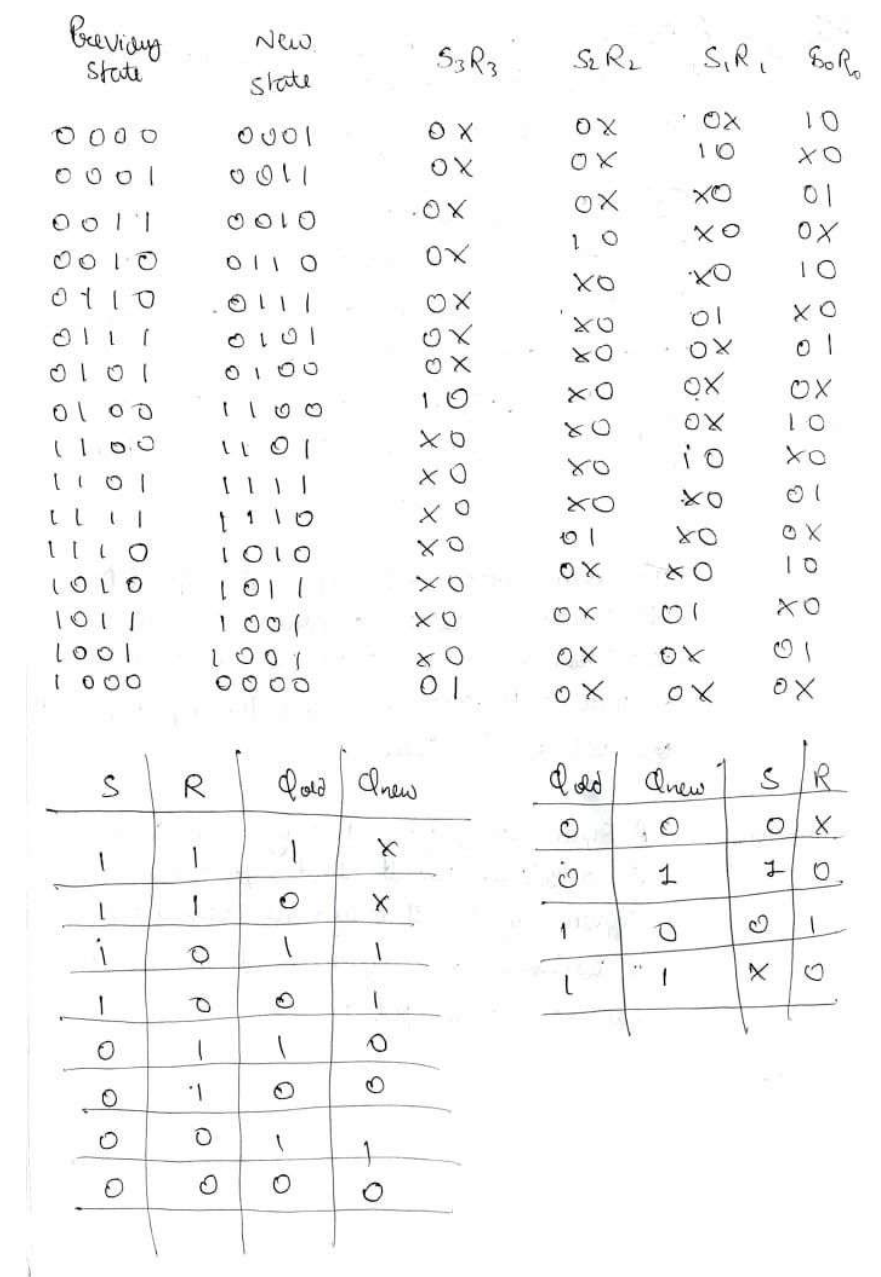
\includegraphics[width=\linewidth]{sr-latch.png}
        \caption{sr-latch}
        \label{fig:enter-label}
    \end{figure}
    \begin{figure}
        \centering
        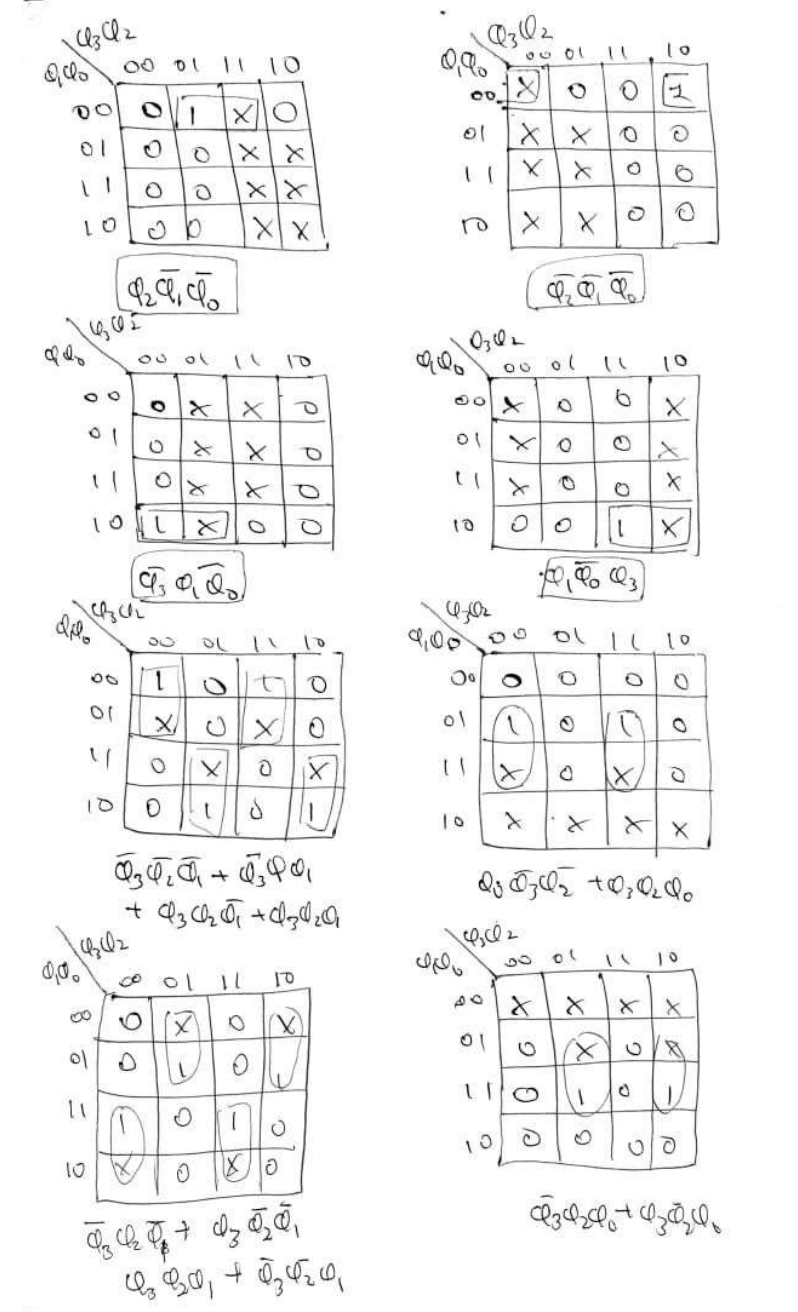
\includegraphics[width=\linewidth]{K-map.png}
        \caption{K-map}
        \label{fig:enter-label}
    \end{figure}


   \newpage 
    \begin{multicols}{2}
    
    \fcolorbox{black}{white}{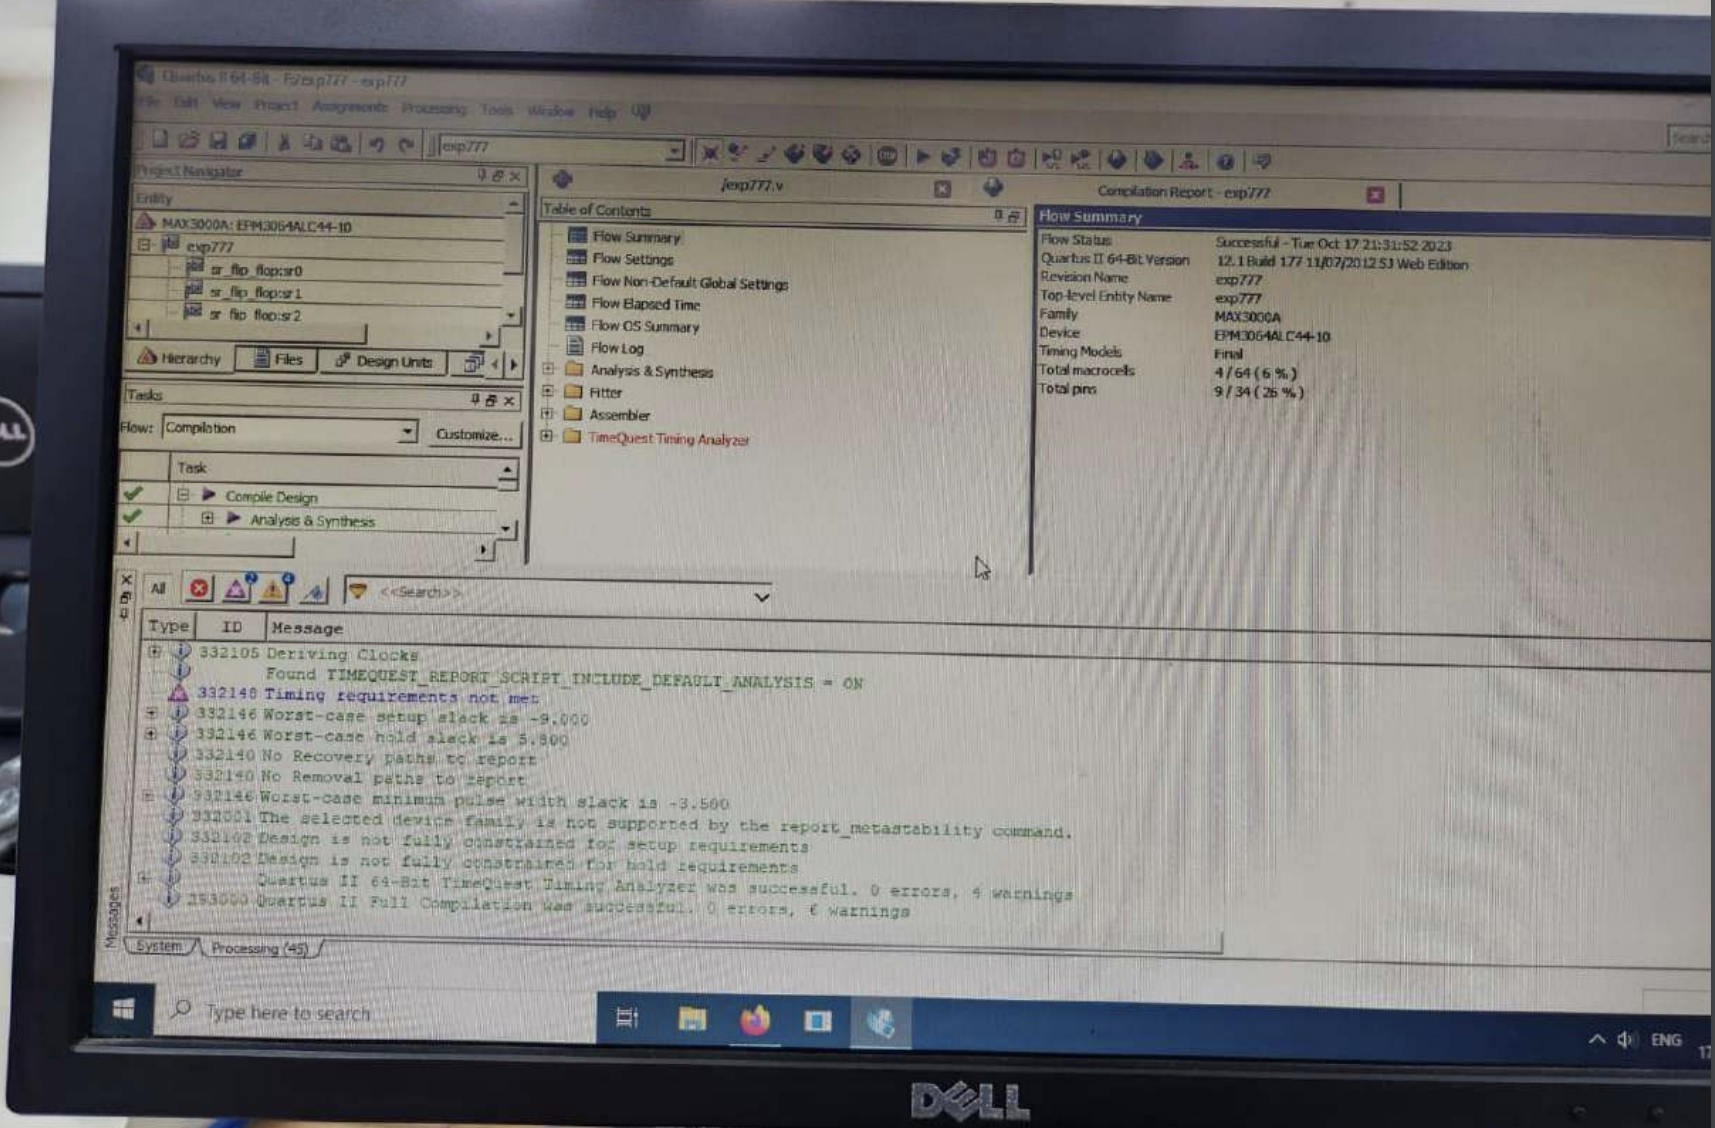
\includegraphics[width=0.9\linewidth]{settings.png}}
    \columnbreak
    \fcolorbox{black}{white}{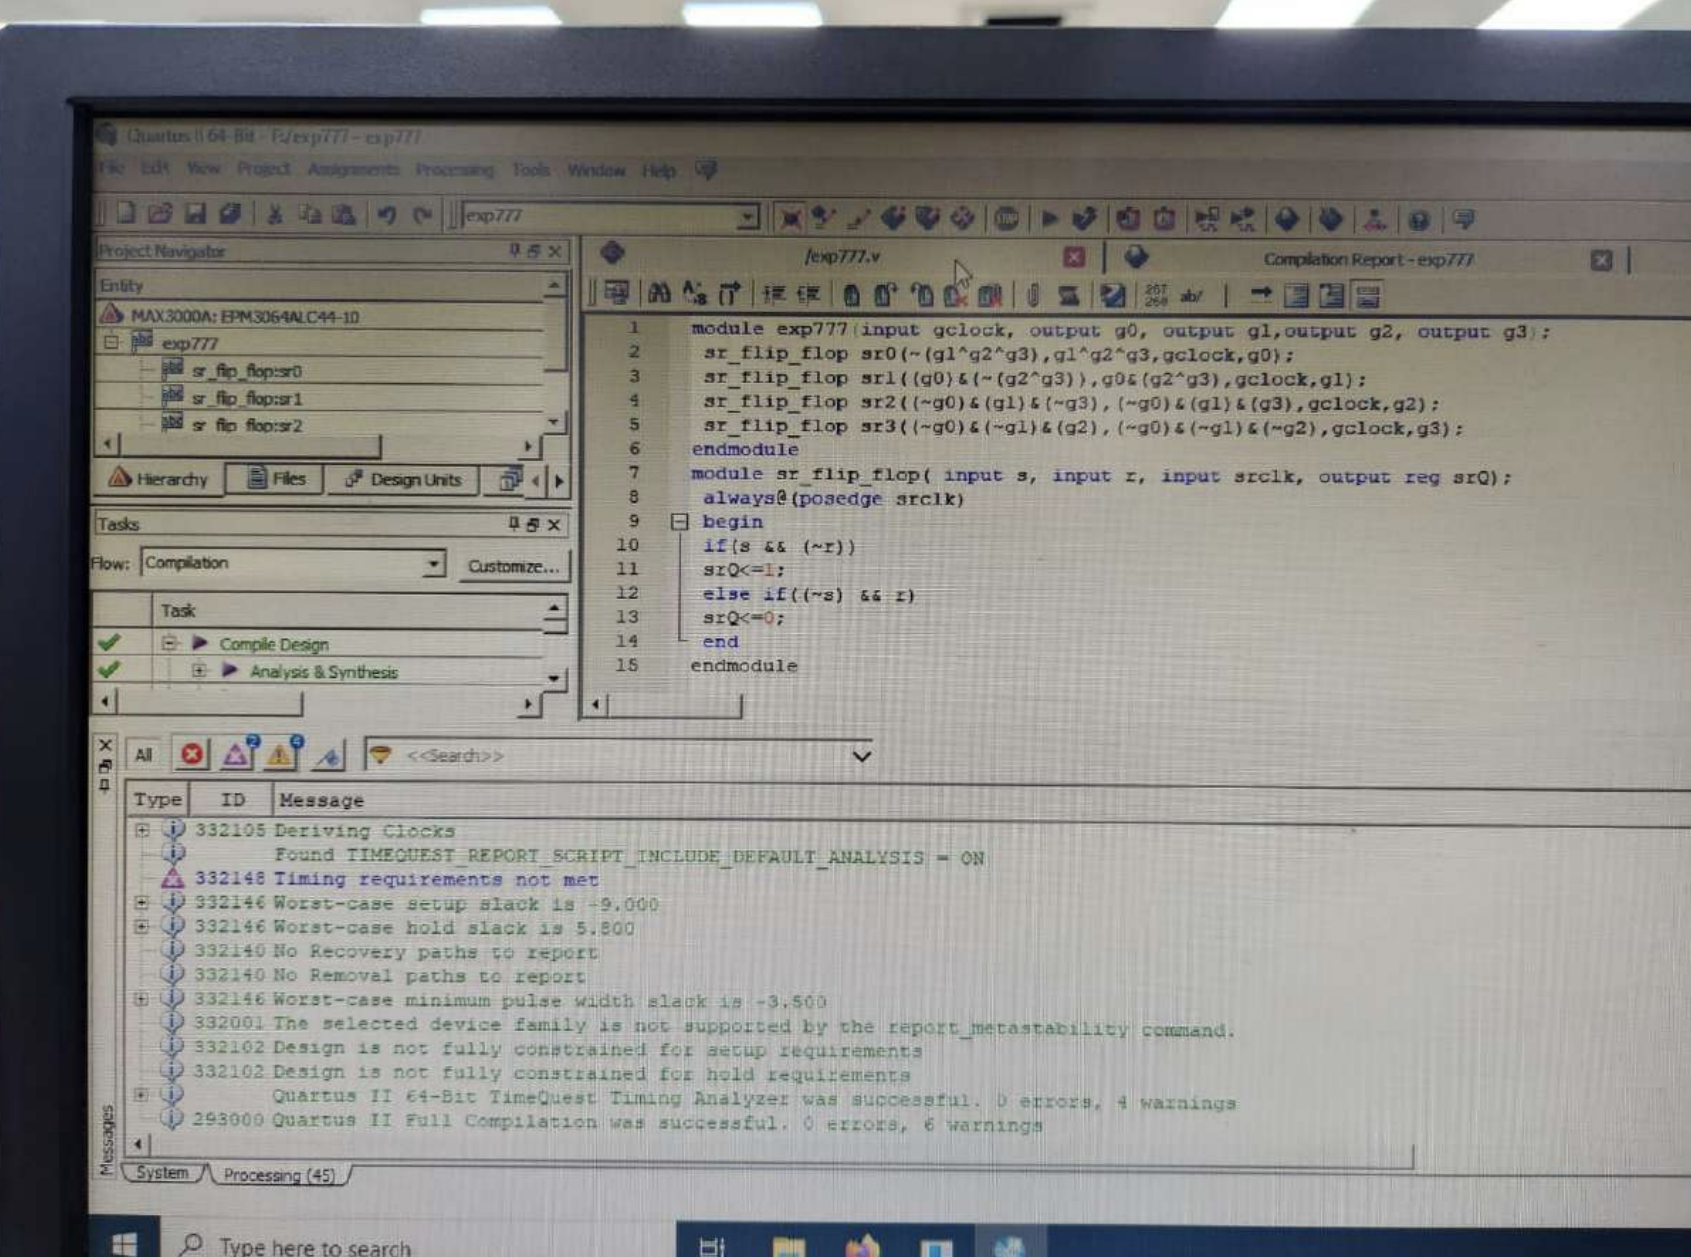
\includegraphics[width=0.8\linewidth]{code.png}}
    \end{multicols}

     \begin{figure}[h!]
        \centering
        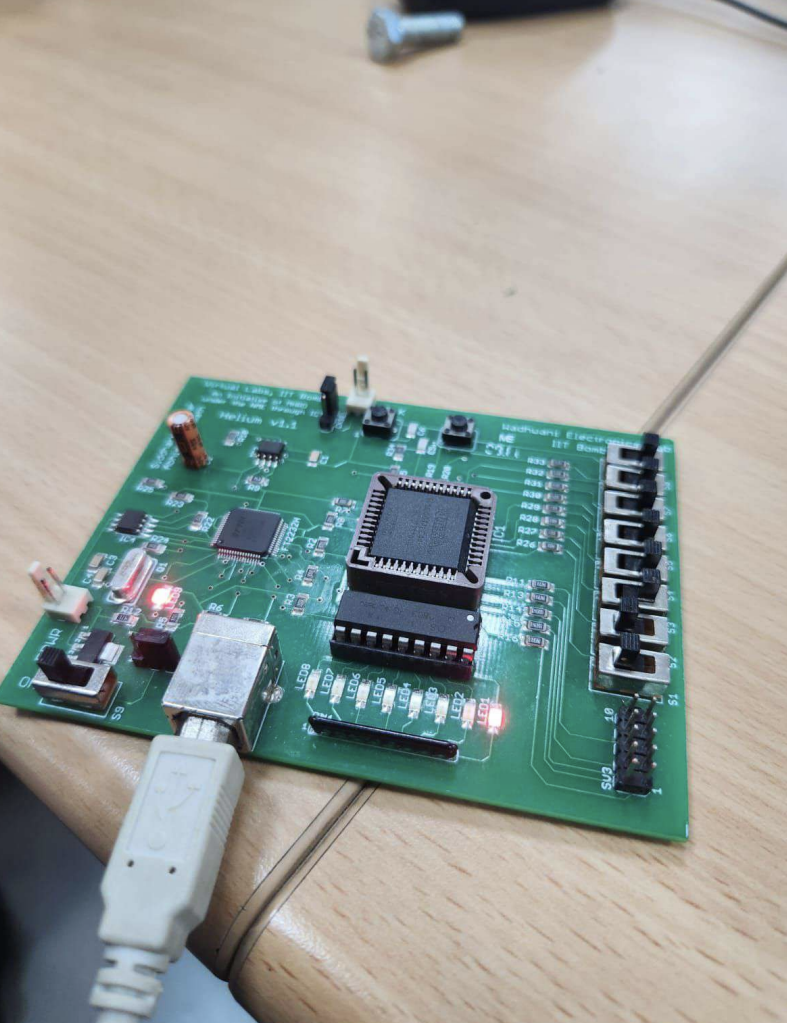
\includegraphics[width=0.5\linewidth]{cpld.png}
        \caption{CPLD}
        \label{fig:enter-label}
    \end{figure}
    
    
    
    
    

    
\section{Conclusions}
    The main idea is to use SR Flip flop. we needed to design a circuit that can transition from one state to next in a gray code Sequence. Each flip-flop reforesent one bit in counter.
\section{Precautions}
    \begin{enumerate}
        \item Ensure that the clock signals and timing requirements are well-defined and adhered to in your circuit. The timing and synchronization of the clock pulses are crucial for the proper functioning of the flip-flops and the transition between states in the Gray Code sequence.
        \item  Implement a proper reset initialization mechanism for the flip-flops. Ensure that the initial state of the counter is well-defined and known. This is important to start the Gray Code sequence from a known state and prevent any ambiguity in the circuit's behavior.
        \item Take precautions to minimize noise and ensure good signal integrity in the circuit. This includes proper decoupling of power supplies, avoiding signal crosstalk, and maintaining clean and stable power and ground connections.
    \end{enumerate}
\end{document}

